\newpage\subsection*{Answers}

\SolutionsStatement

\begin{enumerate}
	
    \item 
    \begin{enumerate}
    	\item We need $25-u^2 \ge 0$, so the domain is $u \in [-5,5]$. For the range, $\sqrt{25-u^2}$ is between 0 and 5, so $f(u)$ is between $-1$ and $4$. The range is the interval $[-1,4]$. 
        \item Complete the square: $t^2 - 8t +3 = t^2 - 8t +16 - 16 +3 = (t-4)^2 - 13$. The domain is the set of real numbers, and the range is the interval $[-13,\infty)$.
        \item $1+\frac{1}{x - 1}$ is defined for $x \le 0$ and $\sqrt{4 - x^2}$ is defined on $(0,2]$. So the domain of $A$ is the interval $(-\infty,2]$. Range: $[0,2)$. 
    \end{enumerate}

	\begin{center}
		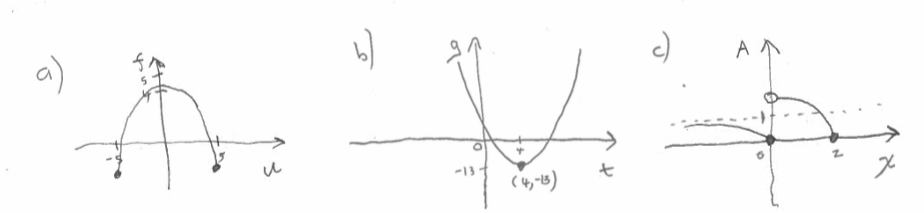
\includegraphics[width=0.8\textwidth]{images/imgWS1Spring17.png} 
	\end{center}

	\item If $\sec \theta = -\sqrt{2}$, then $\cos\theta = -1/\sqrt{2}$, so $\theta = 5\pi/4$. 
    \begin{align*}
    	\cos 5\pi/4 &= -1/\sqrt{2} \\
        \sin 5\pi/4 &= -1/\sqrt{2} \\
        \csc 5\pi/4 &= -\sqrt{2} \\
        \tan 5\pi/4 &= 1 \\
        \cot 5\pi/4 &= 1
    \end{align*}
    \item The purpose of this question to help students become familiar with properties of elementary and rational functions.
    	\begin{enumerate} 
    		\item $2^{-x}$, or $a^{-x}$ for any $a > 0$. 
            \item $|\cos(x)|$, or $|\cos(a x)|$ for any non-zero $a$.
            \item $f(x) = x + 1$.
        \end{enumerate}
       \item Use the identity $\sin (x + y) = \cos x \sin y + \cos y \sin x$. 
       \begin{align*}
       		y &= \frac{\sqrt{3}}{2}\cos(t) + \frac{1}{2}\sin(t) \\
            &= \cos t \sin \frac{\pi}{3} + \cos \frac{\pi}{3} \sin(t) \\
            &= \sin (t + \pi / 3)
       \end{align*}
       \item \begin{align*}
        0 &= \sin2\theta-\cos\theta \\
        &= 2\cos \theta \sin\theta - \cos\theta \\
        &= \cos \theta (2\sin\theta -1)
       \end{align*}
       So either $\cos\theta = 0$ which implies $\theta = \pi/2 + n\pi$, or $\sin\theta = 1/2$, which implies $\theta = \pi/6 + 2n\pi$ and $\theta = 5\pi/6 + 2n\pi$, $n$ is any integer.
       
       
       
       
       
\end{enumerate}